\documentclass[12pt]{extarticle}

\setlength{\headheight}{15pt} % ??? we do what fancyhdr tells us to do  

\title{Physics 2}
\author{Giacomo Ellero}
\date{a.y. 2024/2025}

\usepackage[arrowdel]{physics}
\usepackage{preamble}

% \renewcommand{\vec}[1]{\uvec{#1}}

\begin{document}

\firstpage

\section{Mathematical tools}

\subsection{Scalar and vector fields}

\begin{definition}{Scalar field}{scalar-field}
    A scalar field is a function of type $f:\R^d \to \R$.
\end{definition}

Some examples of scalar fields are temperature or pressure.

\begin{definition}{Level curve of a scalar field}{level-curve-scalar}
    Let $f$ be a scalar field and $k \in \R$ constant.
    Then a level curve of $f$ at $k$ is the set
    \begin{equation}
        \left\{ \vec x \in \R^d : f(\vec x) = k  \right\}
    \end{equation}
\end{definition}


\begin{definition}{Vector field}{vector-field}
    A vector field is a function of type $\vec g: \R^d \to \R^d$.
\end{definition}

Some examples of vector fields are gravitational fields or the velocity field of fluids.

We will always work with \say{well behaved} fields: this means the functions are \say{almost always infinite} (of class $C^\infty$ with only some points as exceptions).

\begin{example}{}{vec-field}
    Let $\vec g(x, y, z) = x \hat x + y \hat y + z \hat z$.

    \begin{figure}[H]
        \centering
        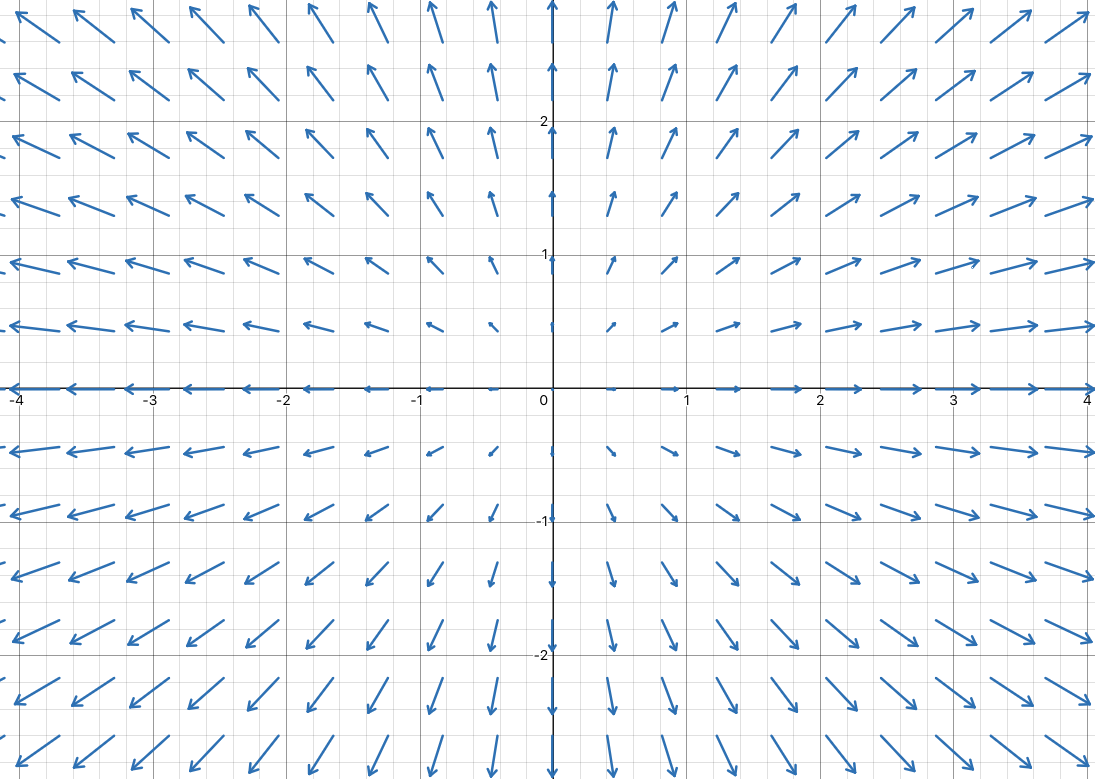
\includegraphics[width=0.6\textwidth]{assets/physics-2/vector-field-example.png}
        \caption{The arrow representation of $\vec g$ when $z = 0$.}
        \label{fig:field_source_0}
    \end{figure}
\end{example}

Some vector fields have \say{special points} where there are an infinite number of field lines going through it:
\begin{itemize}
    \item If all the lines go into that point we call such point \textbf{source} (the point $(0,0,0)$ is a source for \Cref{ex:vec-field});
    \item If all the lines go out of that point we call such point \textbf{sink} (use the field $\vec g(x, y, z) = -x \hat x - y \hat y - z \hat z$ as an example).
\end{itemize}
It is possible for some vector fields to have no sources or sinks. Some patterns that can arise are \textit{loops} or \textit{straight lines}.

\subsection{Operations over fields}

\begin{definition}{Gradient of a scalar field}{gradient-scalar}
    We define the gradient as
    \begin{equation}
        \grad f = \pdv{f}{x} \hat{x} + \pdv{f}{y} \hat{y} + \pdv{f}{z} \hat{z}
    \end{equation}

    We can also define the differential of a field as follows (where $\dd{l} = \dd{x} \hat{x} + \dd{y} \hat{y} + \dd{z} \hat{z} $):
    \begin{equation}
        \dd{f} = \pdv{f}{x} \dd{x} + \pdv{f}{y} \dd{y} + \pdv{f}{z} \dd{z} = \grad f \cdot \dd{\vec l}
    \end{equation}
\end{definition}

The gradient of a field is somewhat the equivalent of the derivative for 1D functions.

\begin{proposition}{Properties of the gradient}{props-gradient}
    \begin{enumerate}[label=\roman*.]
        \item $\grad f$ is orthogonal to the level curves;
        \item $\grad f$ points in the direction of the steepest ascent;
    \end{enumerate}
\end{proposition}

\begin{definition}{Directional derivative}{directional-derivative}
    The directional derivative is the slope of the field in the direction $\vec l$.
    \begin{equation}
        \dv{f}{l} = \grad \cdot \dd{\vec l}
    \end{equation}
\end{definition}

\begin{definition}{Gradient (nabla) operator}{nabla-operator}
    We define the nabla operator as
    \begin{equation}
        \grad = \pdv{}{x} \hat{x} + \pdv{}{y} \hat{y} + \pdv{}{z} \hat{z}
    \end{equation}
\end{definition}

This operator is particularly useful because we can treat it basically like a vector: when we multiply the $\grad$ with a vector field $f$ we get the gradient field of $f$.

\begin{definition}{Divergence}{divergence}
    Let $\vec f$. Then
    \begin{align}
        \div \vec f & = \left( \pdv{}{x} \hat{x} + \pdv{}{y} \hat{y} + \pdv{}{z} \hat{z} \right) \cdot \left( f_x \hat x + f_y \hat y + f_z \hat z\right) \\
                    & = \pdv{f_x}{x} + \pdv{f_y}{y} + \pdv{f_z}{z}
    \end{align}
\end{definition}

The intuition behind divergence is to measure how much a field \say{spreads out} from the point where it si measured.

\begin{example}{}{}
    Take $\vec f$ as in \Cref{fig:field_source_0}. Then
    \begin{equation}
        \div \vec f = \pdv{x}{x} + \pdv{y}{y} + \pdv{z}{z} = 3
    \end{equation}

    We have that the divergence for this field is always positive therefore the arrows always go further away from each other.
\end{example}

\begin{example}{Solenoidal field}{solenoidal-field}
    Let $\vec f = \hat z$. We have $\div \vec f = 0$.

    Fields with zero divergence are called solenoidals.
\end{example}

\begin{definition}{Curl}{curl}
    Let $\vec v$ be a vector field. Then
    \begin{equation}
        \curl \vec f = \det\begin{vmatrix}
            \hat x    & \hat y    & \hat z    \\
            \pdv{}{x} & \pdv{}{y} & \pdv{}{z} \\
            v_x       & v_y       & v_z
        \end{vmatrix}
    \end{equation}
\end{definition}

The intuition behind curl is to measure how much a vector field rotates or spins around the point where we compute it.

\begin{proposition}{Linearity}{linearity-of-grad}
    $\grad(\mathord{\cdot})$, $\div(\mathord{\cdot})$, and $\curl(\mathord{\cdot})$ are linear operators.
\end{proposition}

\begin{proposition}{Leibniz rule}{leibniz-rule}
    \begin{equation}
        \grad{fg} = (\grad f)g + f (\grad g)
    \end{equation}
\end{proposition}

\subsubsection{Higher order derivatives}
\label{sec:higher-order-derivatives}

\begin{enumerate}
    \item \textit{Divergence of gradient} $\div (\grad \vec f)$:

          Also called \textit{laplacian}.
          \begin{equation}
              \div (\grad \vec f) = \pdv[2]{f}{x}
          \end{equation}

    \item \textit{Curl of gradient} $\curl(\grad \vec f)$:
    \item \textit{Gradient of divergence} $\grad (\div \vec f)$:
    \item \textit{Divergence of curl} $\div (\curl \vec f)$:
    \item \textit{Curl of curl} $\curl (\curl \vec f)$:
\end{enumerate}

\subsection{Integrals}

\begin{definition}{Line integral}{line-integral}

\end{definition}

\begin{definition}{Surface integral}{surgace-integral}

\end{definition}

\begin{definition}{Volume integral}{volume-integral}
    Let $f$ be a scalar field and $V \in \R^3$.
    We want to define $I = \int_V f \dd{\tau}$ where $\dd{\tau} = \dd{x} \dd{y} \dd{z}$.

    If $\vec g$ is a vector field we define the integral as
    \begin{equation}
        \vec I = \int_V \vec g(x, y, z) \dd{\tau} = \int_V g_x (x, y, z) \dd{x} \hat x + \int_V g_y (x, y, z) \dd{y} \hat y + \int_V g_z (x, y, z) \dd{z} \hat z
    \end{equation}
\end{definition}

\subsection{Theorems for \texorpdfstring{$\grad(\mathord{\cdot})$, $\div(\mathord{\cdot})$, and $\curl(\mathord{\cdot}) $}{gradient, divergence and curl}}

\begin{theorem}{Fundamental theorem of gradient}{fundamental-gradient}
    Let $f$ be a gradient field and $C$ be a path. We have
    \begin{equation}
        \int_C \dd{f} = \int_A^B \grad f \cdot \dd{\vec l} = f(B)- f(A)
    \end{equation}
\end{theorem}

\begin{corollary}{}{}
    If $\vec v = \grad f$ then $\vec v$ is conservative.
\end{corollary}

\begin{corollary}{}{}
    If $C$ is closed and $\vec v = \grad f$ we have
    \begin{equation}
        \oint \vec v \cdot \dd{\vec l} = \oint \grad f \cdot \dd{l} = 0
    \end{equation}
\end{corollary}

\begin{theorem}{Divergence theorem}{divergence-theorem}
    Let $V$ be a volume, $S$ be a surface corresponding to that volume and $\vec v$ a vector field.
    Then
    \begin{equation}
        \int_V \left(\div \vec v\right) = \oint_S \vec v \cdot \dd{\vec S}
    \end{equation}
\end{theorem}

\begin{proof}
    We have done a partial proof in the case of a cube in Physics 1.
\end{proof}

\begin{corollary}{}{}
    If $\vec v$ is solenoidal
    \begin{enumerate}
        \item $\oint_S \vec v \cdot \dd{\vec S} = 0 \enspace \forall S$
        \item $\int_S \vec v \cdot \dd{S}$ is independent of $S$ but only on the boundary line of $S$
        \item Let $\vec v = \curl \vec A$ where $\vec A$ is a vector field. Then $\div \vec v = \div (\curl \vec A) = 0$
    \end{enumerate}
\end{corollary}

\begin{proof}
    \skiplineafterproof
    \begin{enumerate}
        \item Trivial from theorem and definition of solenoidal.
        \item
              For any $S_1$ open we can find another $S_2$ open with the same boundary line.
              Let $S = S_1 \cup S_2$, then $S$ is closed.
              By the divergence theorem we can write
              \begin{equation}
                  \oint_S \vec v \cdot \dd{\vec S} = \int_V \left(\div \vec v\right) = 0 = \int_{S_1} \vec v \cdot \dd{\vec S} + \int_{S_2} \vec v \cdot \dd{\vec S}
              \end{equation}
              This means that $\abs{\Phi_{S_1}(\vec v)} = \abs{\Phi_{S_2} (\vec v)}$.
        \item This is a consequence of the theorem and the results of \cref{sec:higher-order-derivatives}.
    \end{enumerate}
\end{proof}

\begin{theorem}{Stokes' theorem}{stokes}
    Let $\vec v$ be a vector field, $S$ an open surface, $C$ the boundary line of $S$.
    Then
    \begin{equation}
        \int_S (\curl \vec v) \cdot \dd{\vec S} = \oint_C \vec v \cdot \dd{\vec l}
    \end{equation}
    and the direction of $C$ depends on the direction of the normals of $S$ by the right-hand rule.
\end{theorem}

The intuition behind the theorem is that if we consider the total \say{rotation} in the surface it will be equal to the total \say{diraction} of the vectors at the boundary.

\begin{proof}
    We will consider a surface that can be decomposed in rectangles.
    Consider a rectangle with vertices $P_1,P_2,P_3,P_4$ on the $yz$ plane. Let $\dd{y}$ be the \say{base} of the rectangle, $\dd{z}$ its height and $A = (x, y, z)$ the center of the rectangle.

    Now we want to compute the line integral over the boundary of the rectangle going counterclockwise:
    \begin{align}
        P_1 P_2: \quad & \dd{\vec l} = \dd{y} \hat y \implies \vec v \cdot \dd{\vec l} = v_y\left(x, y, z - \frac{\dd{z}}{2}\right)\dd{y} \approx \left[v_y(x, y, z) \dd{y} - \pdv{v_y(x, y, z)}{z} \frac{\dd{z}}{2}\right] \dd{y}    \\
        P_3 P_4: \quad & \dd{\vec l} = -\dd{y} \hat y \implies \vec v \cdot \dd{\vec l} = -v_y\left(x, y, z - \frac{\dd{z}}{2}\right)\dd{y} \approx -\left[v_y(x, y, z) \dd{y} - \pdv{v_y(x, y, z)}{z} \frac{\dd{z}}{2}\right] \dd{y} \\
        P_2 P_3: \quad & \dd{\vec l} = \dd{z} \hat z \implies \vec v \cdot \dd{\vec l} = v_z\left(x, y - \frac{\dd{y}}{2}, z\right)\dd{y} \approx \left[v_z(x, y, z) \dd{z} - \pdv{v_z(x, y, z)}{y} \frac{\dd{y}}{2}\right] \dd{z}    \\
        P_4 P_1: \quad & \dd{\vec l} = -\dd{z} \hat z \implies \vec v \cdot \dd{\vec l} = -v_z\left(x, y - \frac{\dd{y}}{2}, z\right)\dd{y} \approx -\left[v_z(x, y, z) \dd{z} - \pdv{v_z(x, y, z)}{y} \frac{\dd{y}}{2}\right] \dd{z}
    \end{align}
    where the $\approx$ are due to a taylor expansion.

    By summing up all the terms we get that many terms cancel out:
    \begin{equation}
        P_1P_2 + P_2P_3 + P_3P_4 + P_4P_1 = \left( \pdv{v_z}{y} - \pdv{v_y}{z} \right) \dd{y} \dd{z} = \left( \curl \vec v \right)_x \dd{y} \dd{z}
    \end{equation}

    \textit{A complete proof would require the same procedure on the $xy$ and $xz$ planes.}
\end{proof}

\begin{corollary}{}{}
    The theorem doesn't say anything about $S$ itself, just the boundary $C$.
    Therefore we can say
    \begin{equation}
        \int_S (\curl \vec v) \cdot \dd{\vec S} \text{ only depends on the boundary line of } S
    \end{equation}

    Moreover
    \begin{equation}
        \oint_S (\curl \vec v) \cdot \dd{\vec S} = 0
    \end{equation}
\end{corollary}

\begin{theorem}{Fundamental theorem for irrotational fields}{irrotational-fields}
    Let $\vec v$ such that $\curl \vec v = 0$ everywhere.
    Then:
    \begin{enumerate}
        \item $\oint_C \vec v \cdot \dd{\vec l} \enspace \forall C \text{ closed}$.
        \item $\int_A^B \vec v \cdot \dd{\vec l}$ is independent of the slope of the path.
        \item There exists $f$ such that $\vec v = \grad f$.
    \end{enumerate}
\end{theorem}

\subsection{Dirac delta function}

Let $\vec v = \frac{\vec r}{r^3}$. We want to compute its divergence.
\begin{equation}
    \vec v = \frac{\vec r}{r^3} = \frac{x \hat x + y \hat y + z \hat z}{\left( x^2 + y^2 + z^2\right)^{\frac{3}{2}}} \in \R^3 \setminus (0,0,0)
\end{equation}
\begin{align}
    \pdv{v_x}{x} & = \frac{1}{\left( x^2 + y^2 + z^2\right)^{\frac{3}{2}}} - \frac{3}{2}\frac{2 x^2}{\left( x^2 + y^2 + z^2\right)^{\frac{5}{2}}} = \frac{-2x^2 + y^2 + z^2}{\left( x^2 + y^2 + z^2\right)^{\frac{5}{2}}} \\
    \pdv{v_x}{x} & = \frac{x^2 - 2y^2 + z^2}{\left( x^2 + y^2 + z^2\right)^{\frac{5}{2}}}                                                                                                                                 \\
    \pdv{v_x}{x} & = \frac{x^2 + y^2 - 2z^2}{\left( x^2 + y^2 + z^2\right)^{\frac{5}{2}}}
\end{align}
and by adding up all the partial derivatives we get that $\div \vec v = 0$.

Now let's use the divergence theorem to compute the flux of $\vec v$ over a sphere:
\begin{equation}
    \oint_S \vec v \cdot \dd{\vec S} = \int_V \div \cdot \vec v \dd{\tau} {\color{red}= 0}
\end{equation}

This would look correct but let's also compute this without the divergence theorem.
Using spherical coordinates we write
\begin{equation}
    \dd{\vec S} = \dd{S}\hat r = R^2 \sin\theta \dd{\theta} \dd{\phi} \hat r
\end{equation}
Now we notice that $\dd{S}$ is always at the same distance from the center of the sphere and
\begin{equation}
    \oint_S \vec v \cdot \dd{\vec S} = \int \frac{R}{R^3} \dd{S} = \frac{1}{R^2} \int \dd{S}
\end{equation}
which is equal to the area of the sphere, therefore we get a result of $4\pi$ which conflicts with the result we got from the divergence theorem.

\section{Electric phenomena}

\section{Magnetic phenomena}

\end{document}
